% Options for packages loaded elsewhere
\PassOptionsToPackage{unicode}{hyperref}
\PassOptionsToPackage{hyphens}{url}
%
\documentclass[
  ignorenonframetext,
  10pt,
  xcolor=dvipsnames
]{beamer}

\usepackage{pgfpages}
\setbeamertemplate{caption}[numbered]
\setbeamertemplate{caption label separator}{: }
\setbeamercolor{caption name}{fg=normal text.fg}
\beamertemplatenavigationsymbolsempty
% Prevent slide breaks in the middle of a paragraph
\widowpenalties 1 10000
\raggedbottom
\setbeamertemplate{part page}{
  \centering
  \begin{beamercolorbox}[sep=16pt,center]{part title}
    \usebeamerfont{part title}\insertpart\par
  \end{beamercolorbox}
}
\setbeamertemplate{section page}{
  \centering
  \begin{beamercolorbox}[sep=12pt,center]{part title}
    \usebeamerfont{section title}\insertsection\par
  \end{beamercolorbox}
}
\setbeamertemplate{subsection page}{
  \centering
  \begin{beamercolorbox}[sep=8pt,center]{part title}
    \usebeamerfont{subsection title}\insertsubsection\par
  \end{beamercolorbox}
}
\AtBeginPart{
  \frame{\partpage}
}
\AtBeginSection{
  \ifbibliography
  \else
    \frame{\sectionpage}
  \fi
}
\AtBeginSubsection{
  \frame{\subsectionpage}
}
\usepackage{lmodern}
\usepackage{amsmath}
\usepackage{ifxetex,ifluatex}
\ifnum 0\ifxetex 1\fi\ifluatex 1\fi=0 % if pdftex
  \usepackage[T1]{fontenc}
  \usepackage[utf8]{inputenc}
  \usepackage{textcomp} % provide euro and other symbols
  \usepackage{amssymb}
\else % if luatex or xetex
  \usepackage{unicode-math}
  \defaultfontfeatures{Scale=MatchLowercase}
  \defaultfontfeatures[\rmfamily]{Ligatures=TeX,Scale=1}
\fi
% Use upquote if available, for straight quotes in verbatim environments
\IfFileExists{upquote.sty}{\usepackage{upquote}}{}
\IfFileExists{microtype.sty}{% use microtype if available
  \usepackage[]{microtype}
  \UseMicrotypeSet[protrusion]{basicmath} % disable protrusion for tt fonts
}{}
\makeatletter
\@ifundefined{KOMAClassName}{% if non-KOMA class
  \IfFileExists{parskip.sty}{%
    \usepackage{parskip}
  }{% else
    \setlength{\parindent}{0pt}
    \setlength{\parskip}{6pt plus 2pt minus 1pt}}
}{% if KOMA class
  \KOMAoptions{parskip=half}}
\makeatother
\usepackage{xcolor}
\IfFileExists{xurl.sty}{\usepackage{xurl}}{} % add URL line breaks if available
\IfFileExists{bookmark.sty}{\usepackage{bookmark}}{\usepackage{hyperref}}
\hypersetup{
  pdftitle={DoubleML - Double Machine Learning in R},
  pdfauthor={Presenter},
  hidelinks,
  pdfcreator={LaTeX via pandoc}}
\urlstyle{same} % disable monospaced font for URLs
\newif\ifbibliography
\usepackage{graphicx}
\makeatletter
\def\maxwidth{\ifdim\Gin@nat@width>\linewidth\linewidth\else\Gin@nat@width\fi}
\def\maxheight{\ifdim\Gin@nat@height>\textheight\textheight\else\Gin@nat@height\fi}
\makeatother
% Scale images if necessary, so that they will not overflow the page
% margins by default, and it is still possible to overwrite the defaults
% using explicit options in \includegraphics[width, height, ...]{}
\setkeys{Gin}{width=\maxwidth,height=\maxheight,keepaspectratio}
% Set default figure placement to htbp
\makeatletter
\def\fps@figure{htbp}
\makeatother
\setlength{\emergencystretch}{3em} % prevent overfull lines
\providecommand{\tightlist}{%
  \setlength{\itemsep}{0pt}\setlength{\parskip}{0pt}}
\setcounter{secnumdepth}{-\maxdimen} % remove section numbering
\usepackage[default,light,bold]{sourceserifpro}

\usepackage{amsfonts}
\usepackage{amsmath}
\usepackage{amssymb}
\usepackage{mathpazo}
\usepackage{multimedia}
\usepackage{graphicx}
\usepackage{hyperref}
\usepackage{caption}
\usepackage{pgf}
\usepackage{etoolbox} 
\usepackage{textpos} 

\usepackage{multirow}


\makeatletter \preto{\@verbatim}{\topsep=0pt \partopsep=0pt } \makeatother


\setcounter{MaxMatrixCols}{10}


\newenvironment{stepenumerate}{\begin{enumerate}[<+->]}{\end{enumerate}}
\newenvironment{stepitemize}{\begin{itemize}[<+->]}{\end{itemize} }
\newenvironment{stepenumeratewithalert}{\begin{enumerate}[<+-| alert@+>]}{\end{enumerate}}
\newenvironment{stepitemizewithalert}{\begin{itemize}[<+-| alert@+>]}{\end{itemize} }
\newtheorem{assumption}{Assumption}
\newtheorem{blanktheorem}{}
\newtheorem{result}{Result}
\mode<presentation> { \usetheme{boxes} }

\usetheme[block=fill]{metropolis}


\newcommand{\X}{\mathbb{X}}
\newcommand{\R}{\mathbb{R}}
\newcommand{\N}{\mathbb{N}}


\newcommand{\mS}{\mathcal{S}}
\newcommand{\mP}{\mathcal{P}}
\newcommand{\mD}{\mathcal{D}}
\newcommand{\mW}{\mathcal{W}}
\newcommand{\mF}{\mathcal{F}}
\newcommand{\mE}{\mathcal{E}}
\newcommand{\mG}{\mathcal{G}}
\newcommand{\mL}{\mathcal{L}}
\newcommand{\mC}{\mathcal{C}}
\newcommand{\mU}{\mathcal{U}}
\newcommand{\mX}{\mathcal{X}}
\newcommand{\mV}{\mathcal{V}}
\newcommand{\mZ}{\mathcal{Z}}
\newcommand{\mQ}{\mathcal{Q}}

\newcommand{\bP}{\mathbb{P}}
\newcommand{\bE}{\mathbb{E}}
\newcommand{\bEn}{\mathbb{E}_{n}}
\newcommand{\bG}{\mathbb{G}}
\newcommand{\indep}{\mathop{\perp\!\!\!\!\perp}}

\newcommand{\Gn}{\mathbb{G}_n}
\newcommand{\Gnk}{\mathbb{G}_{n_k}}
\newcommand{\Gna}{\mathbb{G}_{n_a}}
\newcommand{\Gnb}{\mathbb{G}_{n_b}}
\newcommand{\Gp}{\mathbf{G}}
\newcommand{\Pn}{\mathbb{P}_n}
\newcommand{\Pp}{\mathbf{P}}
\newcommand{\F}{\mathcal{F}}
\providecommand{\indx}{\alpha}
\newcommand{\Ep}{{\mathrm{E}}}
\newcommand{\barEp}{\bar \Ep}
\renewcommand{\Pr}{{\mathrm{P}}}
\newcommand{\Proj}{{\mathcal{P}_{X[\hat I]}}}
\newcommand{\barf}{\overline{f}}
\newcommand{\barfp}{\overline{f'}}
\newcommand{\Uniform}{{\text{Uniform}}}
\newcommand{\diam}{{\text{diam}}}
\newcommand{\trace}{{\text{trace}}}
\newcommand{\ad}{\overset{\mathrm{a}}{\sim}}


\renewcommand{\hat}{\widehat}
\newcommand{\En}{{\mathbb{E}_n}}
\newcommand{\EnI}{\mathbb{E}_{n,I}}

\renewcommand{\Pr}{{\mathrm{P}}}
\newcommand{\RR}{\mathbb{R}}
\newcommand{\floor}[1]{\left\lfloor #1 \right\rfloor}
\newcommand{\ceil}[1]{\left\lceil #1 \right\rceil}
\newcommand{\semin}[1]{\phi_{{\rm min}}(#1)}
\newcommand{\semax}[1]{\phi_{{\rm max}}(#1)}
\renewcommand{\hat}{\widehat}
\renewcommand{\leq}{\leqslant}
\renewcommand{\geq}{\geqslant}
\newcommand{\sign}{ {\rm sign}}

\newcommand{\ci}{\perp\!\!\!\perp}

\DeclareMathOperator{\pr}{pr}

\DeclareMathOperator{\Corr}{Corr}
\DeclareMathOperator{\Var}{Var}
\DeclareMathOperator*{\argmax}{arg\,max}
\DeclareMathOperator*{\argmin}{arg\,min}

\usepackage{framed}

\definecolor{title}{rgb}{.0,.0,.7}
\definecolor{proposition}{rgb}{.0,.0,.7}
\definecolor{title}{rgb}{.0,.0,.7}
\definecolor{important}{rgb}{0.5,0.,0.}


\definecolor{greenie}{rgb}{0.00,0.71,0.35}

\definecolor{UHHred}{RGB}{226, 0, 26}
\definecolor{UHHblue}{RGB}{0, 156, 209}
\definecolor{UHHgray}{RGB}{59, 81, 91}

\colorlet{mystructure}{UHHred}
\usecolortheme[named=mystructure]{structure}

\titlegraphic{\flushright \pdftooltip{
\includegraphics[width=2cm]{pictures_and_logos/logo.png}}{The logo of the university of Hamburg. A red rectangle containing the text "UHH" (abbreviation for university of Hamburg) and a castle which is used as a symbol in the coat of arms of the city of Hamburg. To the right of the logo, there is written (in German) "Universität Hamburg, DER FORSCHUNG, DER LEHRE, DER BILDUNG".}} 

\addtobeamertemplate{frametitle}{}{
\begin{textblock*}{100mm}(.85\textwidth,-0.75cm)

\includegraphics[width=2cm]{pictures_and_logos/logo.png}
\end{textblock*}
\vspace*{-5pt}%
\par%
\hspace*{-19pt}%
\color{UHHgray!90}\rule[0.5\baselineskip]{0.75\paperwidth}{0.8pt}%
}


\setbeamertemplate{navigation symbols}{}
\setbeamercolor{background canvas}{bg=white}
%\setbeamercolor{footline}{fg=UHHgray, bg=white}
%\setbeamerfont{footline}{size=\fontsize{7}{9}\selectfontbea}
\setbeamercolor{frametitle}{fg=UHHred, bg=white}
\setbeamercolor{progress bar}{fg=UHHred, bg=UHHgray}
\setbeamercolor{date}{fg=UHHgray, bg=white}

\setbeamertemplate{navigation symbols}{}
\ifluatex
  \usepackage{selnolig}  % disable illegal ligatures
\fi


% additional preamble
\usepackage[backend=bibtex8,style=authoryear-comp,maxnames=2,minnames=1,maxbibnames=99,doi=false,url=false,eprint=false,isbn=false,firstinits=true]{biblatex}
\renewcommand{\newunitpunct}{\addcomma\space}
\renewbibmacro{in:}{}
\renewbibmacro*{volume+number+eid}{%
  \printfield{volume}%
  \printfield{number}%
  \setunit{\addcomma\space}%
  \printfield{eid}}
\DeclareFieldFormat*{number}{\mkbibparens{#1}}
%\bibliography{fs_mkbib}
%\bibliography{MscBib}
\bibhang1em
\renewcommand*{\bibfont}{\footnotesize}

\newcommand{\contrItemNormalSize}[3]{
\begin{columns}
\hspace*{12pt}
\begin{column}{0.075\textwidth}
\includegraphics{pictures_and_logos/#2}
\end{column}
\hspace*{-12pt}
\begin{column}{0.075\textwidth}
\includegraphics{pictures_and_logos/#3}
\end{column}
\hspace*{-12pt}
\begin{column}{0.7\textwidth}
{\scriptsize \fullcite{#1}\par}
\end{column}
\end{columns}
}

\newcommand{\contrItemTitle}[3]{
\begin{columns}
\hspace*{12pt}
\begin{column}{0.1\textwidth}
\includegraphics{pictures_and_logos/#2}
\end{column}
\hspace*{-12pt}
\begin{column}{0.1\textwidth}
\includegraphics{pictures_and_logos/#3}
\end{column}
\hspace*{-12pt}
\begin{column}{0.7\textwidth}
{\large  #1 \par}
\end{column}
\end{columns}
}

\newcommand{\pkgDependency}[2]{
\begin{columns}
\begin{column}{0.25\textwidth}
\includegraphics{pictures_and_logos/#1}
\end{column}
\hspace*{-1cm}
\begin{column}{0.65\textwidth}
{#2}
\end{column}
\end{columns}
}

\preto\fullcite{\AtNextCite{\defcounter{maxnames}{99}}}

\bibliography{content/dml_bibliography.bib}

\usepackage{listings}

% Larger itemize symbols
\newcommand\centerbox[1]{$\vcenter{\hbox{#1}}$}
\defbeamertemplate*{itemize item}{custom circle}[1][.45ex]{%
  \centerbox{\tikz\fill (0,0) circle (#1);}}
\defbeamertemplate*{itemize subitem}{custom circle}[1][.4ex]{%
  \centerbox{\tikz\fill (0,0) circle (#1);}}
\defbeamertemplate*{itemize subsubitem}{custom circle}[1][.3ex]{%
  \centerbox{\tikz\fill (0,0) circle (#1);}}

\setbeamertemplate{itemize item}[custom circle]

% box around text for code block
\makeatletter
\newcommand{\boxedText}[1]{
\tikz[baseline={([yshift=-1ex]current bounding box.center)}] \node [fill=UHHgray,rectangle, minimum width=1ex,rounded corners,align=left] {\normalcolor #1};}
\makeatother




\usepackage{pdfcomment}

\title{DoubleML - Double Machine Learning in R}

\author{\vspace*{-10pt}
Philipp Bach, Malte S. Kurz}

\begin{document}
\begin{frame}

\date{}
\institute{
\href{mailto:philipp.bach@uni-hamburg.de}{philipp.bach@uni-hamburg.de} \\
\href{mailto:malte.simon.kurz@uni-hamburg.de}{malte.simon.kurz@uni-hamburg.de}\\ \\
\vspace{30pt}
\pdftooltip{
\begin{beamercolorbox}[wd=\textwidth,rounded=true,shadow=true]{block body example}
\contrItemTitle{UseR! 5-9 July, 2021}{DoubleML_Rhino_1000x1000.png}{userlogo.png}
\end{beamercolorbox}}
{The logos of the DoubleML package and the logo of the UseR! conference together with the text "UseR! 5-9 July, 2021".}
}
\maketitle

\end{frame}


\hypertarget{causal_ml}{%
\section{Introduction to Double Machine Learning}\label{causal_ml}}

\mode<all>
\mode*


\begin{frame}
\frametitle{What is Double Machine Learning (DML)?}
%\begin{itemize}
%\item \textbf{DML} combines econometrics and machine learning
%\item \textbf{Exploiting the strengths of two disciplines}:
%\end{itemize}
%\vspace*{-10pt}
\begin{center}
\pdftooltip{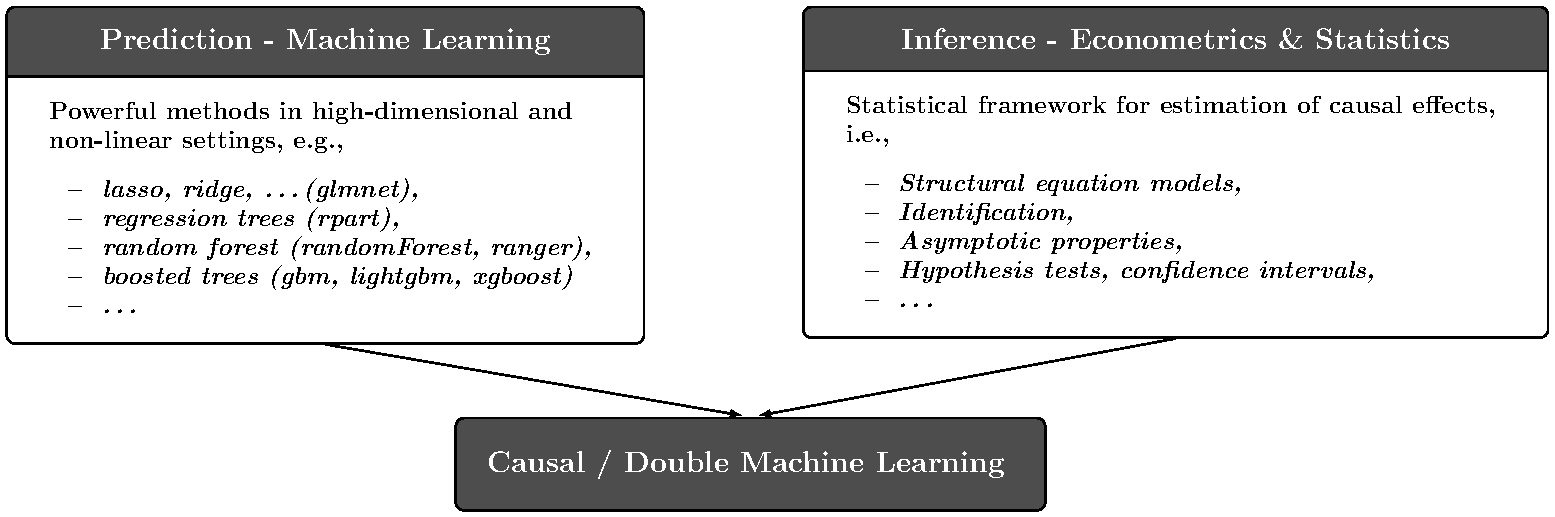
\includegraphics[width = \textwidth]{workflow/doubleml_ml_eco_useR.pdf}}{
A diagram with three boxes. On top, there are two boxes. On the left, a box with title PREDICTION - MACHINE LEARNING; on the right a box with title INFERENCE - ECONOMETRICS AND STATISTICS. In the first box (prediction) it is written: Powerful methods in high-dimensional and non-linear settings, for example, lasso, ridge, regression trees, random forests and boosted trees. In the second box (inference) it is written: Statistical framework for estimation of causal effects, this is, structural equation models, identification, asymptotic theory, hypothesis tests and confidence intervals.}
\end{center}
%\begin{itemize}
%\item \textbf{Machine Learning}: Prediction in high-dimensional non-linear settings
%\item \textbf{Econometrics}: Causality, identification, asymptotic properties of estimators
%\end{itemize}
\begin{itemize}
\item \textbf{Result / output} from the DML framework:
\begin{itemize}
\item Estimate of a causal effect or structural parameter with valid confidence intervals $\rightarrow$ statistical tests for parameter(s) of interest
\item Good statistical properties ($\sqrt{N}$ rate of convergence; unbiased; approximately Gaussian)
%\item Multiple treatment effects; heterogeneous treatment effects, \ldots
\end{itemize}
\end{itemize}
\end{frame}


\begin{frame}
\frametitle{Causal Machine Learning: Examples}
\begin{itemize}
\item Evaluation of an intervention in randomized controlled trials or observational studies, e.g., A/B testing, clinical studies, program evaluation
\item General: What is the \textbf{effect} of a certain \textbf{treatment} on a relevant \textbf{outcome} variable?
%\item A \textbf{randomized experiment} is a direct way to estimate a \textbf{causal effect} (assuming it is conducted properly)
\vspace{10pt}
\end{itemize}
\begin{center}
\pdftooltip{
\includegraphics[width=0.4\textwidth]{pictures_and_logos/ab_testing.jpg}}{An illustration of A/B testing. Stylized persons look on a split screen. On the left hand side of the screen there is a window with an orange rectangle (illustrating version A). On the right hand side of the screen there is a window with a yellow rectangle (illustrating version B). To the left of the screen there is a graph with an increasing red curve and a check mark above. On the right of the screen, there is stagnating yellow graph and a cross above.}
\end{center}
{\tiny \hfill Image Source: Freepik (\url{http://www.freepik.com}) / Designed by macrovector}
\end{frame}

%\begin{frame}
%\frametitle{Example: Partially Linear Regression}
%\begin{itemize}
%\item Partially linear regression (PLR) model
%\begin{align*}
%Y = D\theta_0 + g_0(X) + \zeta, \quad \mathbb{E}(\zeta|D,X)=0,
%\end{align*}
%with potentially non-linear function $g_0(X)$ and 
%\begin{itemize}
%\item $Y$ - outcome variable,
%\item $D$ - treatment variable, 
%\item $X = (X_1,\ldots, X_p)$ - potentially high-dimensional vector of confounding variables.
%\end{itemize}
%\end{itemize}
%\vspace{10pt}
%\begin{center}
%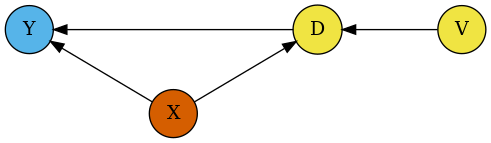
\includegraphics[width=0.6\textwidth]{pictures_and_logos/dag_plr2.png}
%\end{center}
%\end{frame}
%


\mode<all>
\mode*

\begin{frame}
\frametitle{Example: Partially Linear Regression}
%\begin{block}{Partially Linear Regression model (PLR)}
%\textbf{Partially linear regression} models take the form

\begin{itemize}
\item Partially linear regression (PLR) model
\begin{align*}
&Y = D \theta_0 + g_0(X) + \zeta, & &\mathbb{E}[\zeta | D,X] = 0, 
\end{align*}
with potentially non-linear function $g_0()$ and
%\vspace*{-20pt}
%\end{block}
\begin{itemize}
\item Outcome variable $Y$
\item Policy or treatment variable of interest $D$
\item High-dimensional vector of confounding covariates $X = (X_1, \ldots, X_p)$
%\item Stochastic errors $\zeta$ and $V$
\end{itemize}
\end{itemize}
%\vspace{10pt}
%\begin{center}
%\pdftooltip{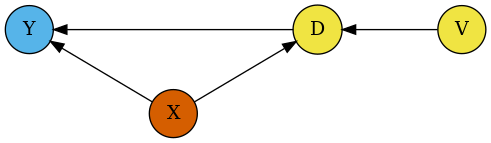
\includegraphics[width=0.6\textwidth]{pictures_and_logos/dag_plr2.png}}{A graph illustrating the  partially linear regression setting. There are four nodes in total: One for the dependent variable Y, one for the treatment variable D, one for the vector of confounding variables X and one for the stochastic error V. There are four directed edges in the figure, each illustrating a causal channel: From V into D, from D into Y, from X into Y and from X into D.}
%\end{center}
\end{frame}

\begin{frame}
\frametitle{Problems in Naive Approaches}
\begin{itemize}
\item Failure of naive approaches: \textbf{Regularization bias}, e.g.,
\begin{itemize}
\item Naive variable selection, for example based on the lasso
\item Naive plug-in predictions, for example from random forests
\end{itemize}
\end{itemize}
\vspace{10pt}
\begin{center}
\pdftooltip{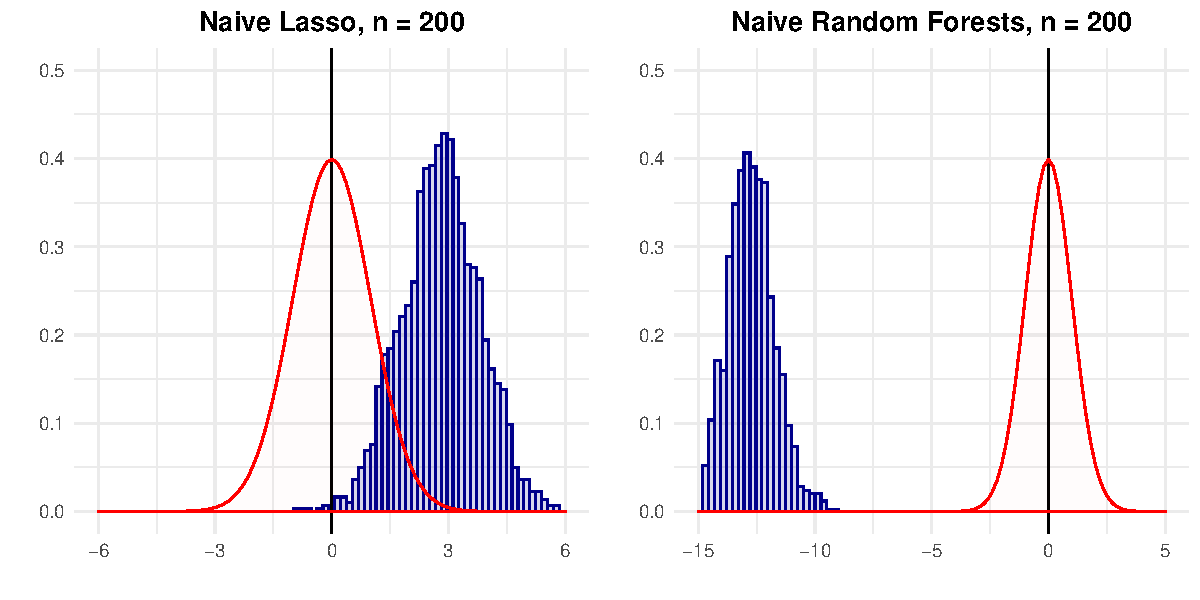
\includegraphics[width=0.8\textwidth]{pictures_and_logos/comp_naive_ml_resc_n200_p200.pdf}}{The figure shows two histograms of the empirical distribution (blue bars) of two naive machine learning estimators for THETANULL in a simulation example. The estimators are studentized, i.e., the true value of THETANULL is subtracted from the value of the estimator and this difference is then divided by the empirical standard deviation of the simulated estimators. The histogram on the left hand side corresponds to estimation of THETANULL that is based on naive variable selection by the lasso, i.e., only those variables in the PLR are included that have been selected in a lasso regression. The histrogram on the right hand side corresponds to a random forest learner which is trained to generate predictions for the outcome Y using covariates X. These predictions are then simply plugged in into the PLR regression equation. In both cases the empirical distribution substantially differs from a normal distribution. In both figures, the density of a standard normal random variable is illustrated by a red curve, which is symmetric around zero. As opposed to the shape of this density, both histograms are not centered at zero, which illustrates a severy bias. In case of the lasso, the estimator is upward biased and in case of the random forest estimator, the estimator is downward biased. Moreover the empirical distributions do not appear symmetric.}
\end{center}
\end{frame}


%\begin{frame}
%\frametitle{Data Generating Process}
%\begin{itemize}
%\item \textbf{Partially linear regression} model
%\vspace*{-10pt}
%\begin{align*}
%&y_i = d_i \theta_0 + g_0(x_i) + \zeta_i, \\
%&d_i = m_0(x_i) + v_i,
%\end{align*}
%with $\zeta_i, v_i \sim \mathcal{N}(0,1)$ and $x_i \sim \mathcal{N}_{p}(0, \Sigma)$.
%\item Variance-covariance matrix $\Sigma$ with entries $\Sigma_{kj} = 0.7^{|j-k|}$
%\item True parameter $\theta_0 = 0.5$
%\item \textbf{Non-linear nuisance functions}
%\vspace*{-5pt}
%\begin{align*}
%&g_0(x_i) = \frac{\exp(x_{i1})}{1+\exp(x_{i1})} + \frac{1}{4} x_{i3} \\
%&m_0(x_i) = x_{i1} + \frac{1}{4} \frac{\exp(x_{i3})}{1+\exp(x_{i3})}
%\end{align*}
%\item $n=500$ observations and $p=20$ explanatory variables
%\end{itemize}
%\end{frame}
%
%
%
%\begin{frame}
%\frametitle{Regularization Bias in Simple ML-Approaches}
%\textbf{Naive} prediction-focused \textbf{ML approach} (Don't do it!):
%\begin{itemize}
%\item Fit a random forest (or another ML method) to predict $Y$ based on the features $X$, i.e., estimate $g_0(X)$
%\item Given $\hat{g}_0(X)$, the final estimate of $\theta_0$ is obtained as ($n=N/2$)
%\end{itemize}
%\vspace*{-7pt}
%\begin{align*}
%\hat{\theta}_0 = \left(\frac{1}{n} \sum_{i\in I} D_i^2\right)^{-1} \frac{1}{n} \sum_{i\in I} D_i (Y_i - \hat{g}_0(X_i))
%\end{align*}
%\vspace*{-7pt}
%\begin{itemize}
%\item Driving factor for the \textbf{regularization bias}: \textbf{Bias in learning $g_0$}
%\end{itemize}
%\begin{columns}
%\hspace*{12pt}
%\begin{column}{0.5\textwidth}
%\includegraphics[height=0.75\textwidth]{../../../paper_py_pkg/sim/presentation/predictions.png}
%\end{column}
%\begin{column}{0.5\textwidth}
%\includegraphics[height=0.75\textwidth]{../../../paper_py_pkg/sim/presentation/nonorth.png}
%\end{column}
%\end{columns}
%\end{frame}

%
%\begin{frame}
%\frametitle{Overcoming Regularization Bias by \\Orthogonalization}
%\begin{itemize}
%\item Directly \textbf{partialling out} the effect of $X$ from $D$ to obtain the \textbf{orthogonalized} regressor $V = D - m_0(X)$
%\item Use the final estimate
%\begin{align*}
%\hat{\theta}_0 = \left(\frac{1}{n} \sum_{i\in I} \hat{V}_i \hat{V}_i\right)^{-1} \frac{1}{n} \sum_{i\in I} \hat{V}_i (Y_i - \hat{g}_0(X_i))
%\end{align*}
%\end{itemize}
%\begin{center}
%\includegraphics[width = 0.45\textwidth]{../../../paper_py_pkg/sim/presentation/orth.png}
%\end{center}
%\end{frame}
%
%\begin{frame}
%\frametitle{Sample Splitting to Remove Bias Induced \\by Overfitting}
%\begin{itemize}
%\item If the nuisance models $\hat{g}_0$ and $\hat{m}_0$ are estimated on the whole dataset, which is also used for obtaining the final estimate $\hat{\theta}_0$, another \textbf{bias induced by overfitting} can be observed
%\end{itemize}
%\begin{center}
%\includegraphics[width = 0.45\textwidth]{../../../paper_py_pkg/sim/presentation/nosplit.png}
%\end{center}
%\end{frame}
%
%
%\begin{frame}
%\frametitle{Sample Splitting to Remove Bias Induced \\by Overfitting}
%\begin{itemize}
%\item Use \textbf{sample splitting} to overcome the \textbf{bias induced by overfitting}, i.e.,
%\begin{itemize}
%\item Estimate the nuisance models $\hat{g}_0$ and $\hat{m}_0$ on one part of the data (training data)
%\item Estimate $\hat{\theta}_0$ on the other part of the data (test data)
%\end{itemize}
%\end{itemize}
%\begin{center}
%\includegraphics[width = 0.45\textwidth]{../../../paper_py_pkg/sim/presentation/dml.png}
%\end{center}
%\end{frame}
%
%\begin{frame}
%\frametitle{Sample Splitting to Remove Bias Induced \\by Overfitting}
%\begin{itemize}
%\item \textbf{Cross-fitting} performs well empirically (efficiency gain by switching roles)
%\end{itemize}
%\begin{columns}
%\hspace*{12pt}
%\begin{column}{0.5\textwidth}
%\includegraphics[height=0.8\textwidth]{../../../paper_py_pkg/sim/presentation/orth_theta.png}
%\end{column}
%\begin{column}{0.5\textwidth}
%\includegraphics[height=0.8\textwidth]{../../../paper_py_pkg/sim/presentation/dml_theta.png}
%\end{column}
%\end{columns}
%\end{frame}
%
%
%\begin{frame}
%\frametitle{Comparison of All Approaches}
%
%\begin{center}
%\includegraphics[width=0.95\textwidth]{../../../paper_py_pkg/sim/presentation/all.png}
%\end{center}
%\end{frame}



\mode<all>
\mode*


\begin{frame}
\frametitle{What is Double Machine Learning (DML)?}
\begin{itemize}
\item \textbf{Double/debiased machine learning (DML)} \parencite{Chernozhukov2018}:  General framework for estimation of treatment effects based on machine learning (ML)
\item The parameter of interest, $\theta_0$, is identified as the solution to a moment condition 
\begin{align*}
\mathbb{E}\left[\psi(W;\theta_0, \eta_0 \right)] = 0,
\end{align*}
with score function $\psi(\cdot)$, i.i.d. data $W$ and nuisance term $\eta$.
\item \textbf{Key ingredients} of the DML approach
\begin{enumerate}
\item Neyman orthogonality,
\item High-quality machine learning estimators,
\item Sample splitting.
\end{enumerate}
%
%\item Combines the strength of \textbf{machine learning} and \textbf{econometrics}
%\item Our object-oriented implementation \textbf{DoubleML} (in \texttt{R} and \texttt{Python}) provides a general interface for the growing number of models and methods for DML
%\item The \texttt{R} package is available on \href{https://cran.r-project.org/web/packages/DoubleML/index.html}{\textbf{CRAN}}.
\end{itemize}
\end{frame}


\mode<all>
\mode*

\begin{frame}
\frametitle{The Key Ingredients of DML}
\begin{block}{1. Neyman Orthogonality}
\begin{itemize}
\item An essential property of the score is \textbf{Neyman orthogonality}
\begin{align*}
\left.\partial_\eta \mathbb{E}[\psi(W; \theta_0, \eta)] \right|_{\eta=\eta_0} = 0.
\end{align*}
\item The moment condition identifying $\theta_0$ is \textit{insenstive to small pertubations of} $\eta$ \textit{around} $\eta_0$. $\Rightarrow$ Estimation \textit{immunized} against first order biases from replacing $\eta_0$ by ML estimator $\hat{\eta}_0$.
\end{itemize}
\end{block}
\begin{itemize}
\item PLR example: Inclusion of first-stage regression
\begin{align*}
D = m(X) + V, 
\end{align*}
leads to the Neyman-orthogonal score
\begin{align*}
\psi(W;\theta, \eta) := \left(Y-g(X) - \theta D \right)\left(D-m(X) \right),
\end{align*}
with $\eta=\left\{g,m \right\}$.
\end{itemize}

\end{frame}


\begin{frame}
\frametitle{The Key Ingredients of DML}
\begin{block}{2. High-Quality Machine Learning Estimators}
The nuisance parameters are estimated with high-quality machine learning methods, i.e., $\eta_0$ is estimated at a sufficiently fast rate of convergence.
\end{block}
\begin{itemize}
\item Different structural assumptions on $\eta_0$ lead to the use of different machine-learning tools for estimating $\eta_0$
\end{itemize}

\begin{block}{3. Sample Splitting}
To avoid the biases arising from overfitting, a form of \textbf{sample splitting} is used at the stage of producing the estimator of the main parameter $\theta_0$.
\end{block}
\begin{itemize}
\item Fit ML models on \textit{train sample}, generate predictions on \textit{test sample}. Swap the roles to gain full efficiency (cross-fitting). Plug in predictions into the score and solve for $\theta_0$
\end{itemize}
\end{frame}
%
%\begin{frame}{Main Result}
%\protect\hypertarget{main-result}{}
%\footnotesize
%
%\begin{block}{\footnotesize Main Result for DML Estimation}
%There exist regularity conditions such that:
%\begin{itemize}
%\item The DML estimator $\tilde{\theta}_0$ concentrates in a $1/\sqrt{N}$-neighborhood of $\theta_0$.
%\item The sampling error $\sqrt{N}(\tilde{\theta}_0 - \theta_0)$ is approximately normal
%\begin{align*}
%\sqrt{N}(\tilde{\theta}_0 - \theta_0) \leadsto N(0, \sigma^2),
%\end{align*}
%with mean zero and variance given by 
%\begin{align*}
%\begin{aligned}\sigma^2 &= J_0^{-2} \mathbb{E}(\psi^2(W; \theta_0, \eta_0)),\\
%J_0 &= \mathbb{E}(\psi_a(W; \eta_0)),\end{aligned}
%\end{align*}
%based on a linear score $\psi(W;\theta, \eta) = \psi_a(W; \eta) \theta + \psi_b(W; \eta)$.
%\end{itemize}
%\end{block}
%\end{frame}

\begin{frame}{The Double Machine Learning Framework}

\begin{itemize}
\item Under regularity conditions, it can be shown that
\begin{align*}
\sqrt{N}(\tilde{\theta}_0 - \theta_0) \leadsto N(0, \sigma^2).
\end{align*}
\item For more details, see \textcite{Chernozhukov2018} and the  \href{https://arxiv.org/abs/2103.09603}{\textbf{package vignette}} \parencite{bach2021doublemlR}
\end{itemize}
\vspace{10pt}
\begin{center}
\pdftooltip{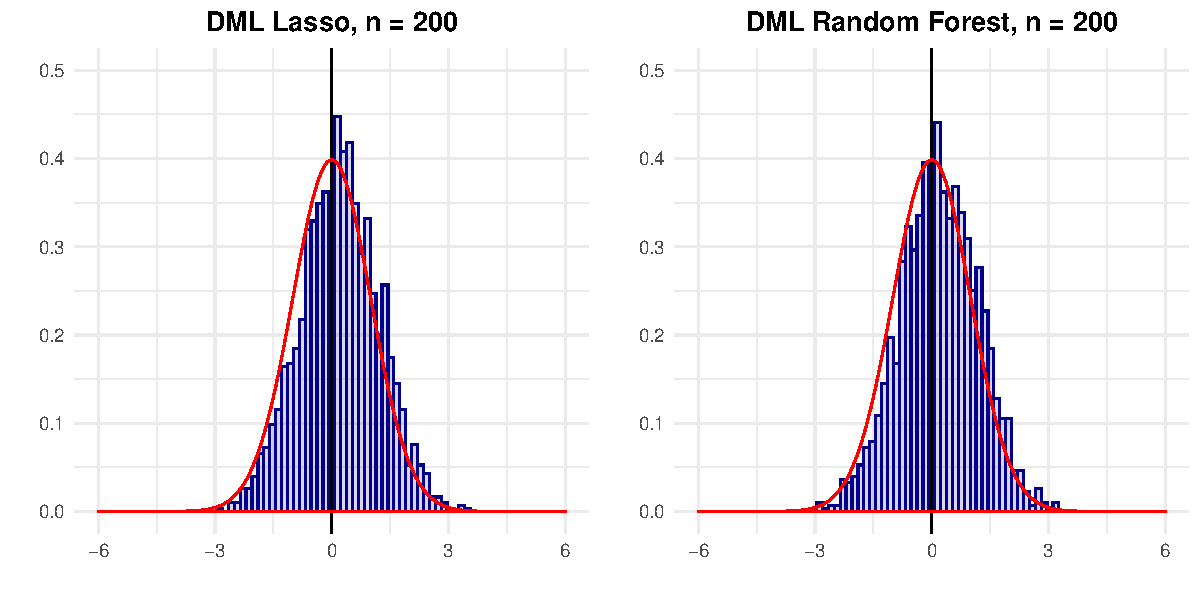
\includegraphics[width=0.8\textwidth]{pictures_and_logos/DMLcomp_dml_resc_n200_p200.pdf}}{ The figure shows two histograms of the empirical distribution (blue bars) of two double machine learning estimators for THETANULL in a simulation example. The estimators are studentized, i.e., the true value of THETANULL is subtracted from the value of the estimator and this difference is then divided by the empirical standard deviation of the simulated estimators. The histogram on the left hand side corresponds to a DML learner that is based on a lasso learner. The histogram on the right hand side corresponds to a DML learner that is based on a random forest. In both figures, the density of a standard normal random variable is illustrated by a red curve, which is symmetric around zero. The empirical distribution of both DML estimators is very similar to the standard normal density which should illustrate the validity of the double machine learning approach.}
\end{center}

\end{frame}



\begin{frame}[noframenumbering, plain]
\hypertarget{packages}{%
\section{The R Package DoubleML}\label{packages}}
\begin{center}
\pdftooltip{
\includegraphics[width=0.3\textwidth]{pictures_and_logos/DoubleML_Rhino_1000x1000.png}}{The logo of the DoubleML package: A two-headed rhino which is a doubly robust animal.}
\end{center}
\end{frame}

\mode<all>
\mode*

\begin{frame}
\frametitle{The R Package DoubleML:\\ Building Principles}

\begin{block}{DoubleML -  Building Principles}
\footnotesize
\begin{tabular}{l l c}
\multirow{2}{*}{\textbf{Key ingredient}} &\multirow{2}{*}{\textbf{Implementation}} & \multirow{2}{*}{ \pdftooltip{
\includegraphics[width=0.09\textwidth]{pictures_and_logos/DoubleML_Rhino_1000x1000.png}}{The logo of the DoubleML package for R.} } \\ & &  \\ & & \\[-0.8ex]
1. Orthogonal score &  Object-oriented implementation & \multirow{4}{*}{ \pdftooltip{\includegraphics[width=0.07\textwidth]{pictures_and_logos/R6.png}}{The logo of the R6 package for R.} }  \\
                    &  with \texttt{R6}; exploit common structure & \\
                    & centered around a (linear) score  &\\ & function $\psi(\cdot)$ & \\  & & \\[-0.8ex]
2. High-quality ML & State-of-the art ML prediction \& tuning  &  \multirow{5}{*}{ \pdftooltip{
\includegraphics[width=0.08\textwidth]{pictures_and_logos/mlr.png}}{The logo of the mlr3 package for R.} }  \\
                   & methods provided by \texttt{mlr3} ecosystem & \\
                   & (meta packages) &\\  & & \\[-0.8ex]
3. Sample splitting & Built-in resampling schemes of \texttt{mlr3} & \\
\end{tabular}
\end{block}
\end{frame}


\begin{frame}
\frametitle{The R Package DoubleML:\\ Main Dependencies and Installation}
\vspace*{-10pt}
%\begin{columns}[t]
%\begin{column}{0.4\textwidth}
\begin{block}{\pdftooltip{Dependencies}{A box containing the names of the main dependencies of the DoubleML package together with their logos. These are the packages mlr3, R6, data.table, mlr3learners and mlr3tuning.}}
\vspace{8pt}
\begin{columns}[t]
\begin{column}{0.25\textwidth}
\pkgDependency{mlr.png}{\texttt{mlr3}} 
\vspace{8pt}
\pkgDependency{mlr.png}{\texttt{mlr3learners}}
\end{column}
\begin{column}{0.25\textwidth}
\pkgDependency{r6.png}{\texttt{R6}}
\vspace{8pt}
\pkgDependency{mlr.png}{\texttt{mlr3tuning}}
\end{column}
\begin{column}{0.25\textwidth}
\pkgDependency{datatable.png}{\texttt{data.table}} 
\end{column}
\end{columns}
\end{block}
\vspace{10pt}
%\end{column}
%\begin{column}{0.6\textwidth}
\begin{block}{Installation}
\begin{itemize}
\item \textbf{Latest} CRAN \textbf{release} \\
\boxedText{\textcolor{white}{\texttt{\footnotesize \$ install.packages('DoubleML')}}}
\item \textbf{Development version} from GitHub \\
\boxedText{\textcolor{white}{\texttt{\footnotesize \$ remotes::install\_github('DoubleML/doubleml-for-r')}}}
\end{itemize}
\end{block}
%\end{column}
%\end{columns}
\end{frame}


\begin{frame}
\frametitle{Why an Object-Orientated Implementation?}
\begin{itemize}
\item Given the components ($\psi^a(\cdot)$ \& $\psi^b(\cdot)$) of a linear Neyman orthogonal score function $\psi(\cdot)$, a \textbf{general implementation} is possible for
\begin{itemize}
\item The estimation of the \textbf{orthogonal parameters}
\item The computation of the \textbf{score} $\psi(W; \theta, \eta)$
\item The estimation of \textbf{standard errors}
\item The computation of \textbf{confidence intervals}
\item A \textbf{multiplier bootstrap} procedure for simultaneous inference
\end{itemize}
\item The \textbf{sample splitting} can be implemented in general as well
\end{itemize}
$\rightarrow$ Implemented in the \textbf{abstract base class} \texttt{DoubleML}
\begin{itemize}
\item The \textbf{score components} and the estimation of the \textbf{nuisance models} have to be implemented \textbf{model-specifically}
\end{itemize}
$\rightarrow$ Implemented in \textbf{model-specific classes} inherited from \texttt{DoubleML}
\end{frame}


\begin{frame}
\frametitle{Class Structure and Causal Models}
\begin{center}
\pdftooltip{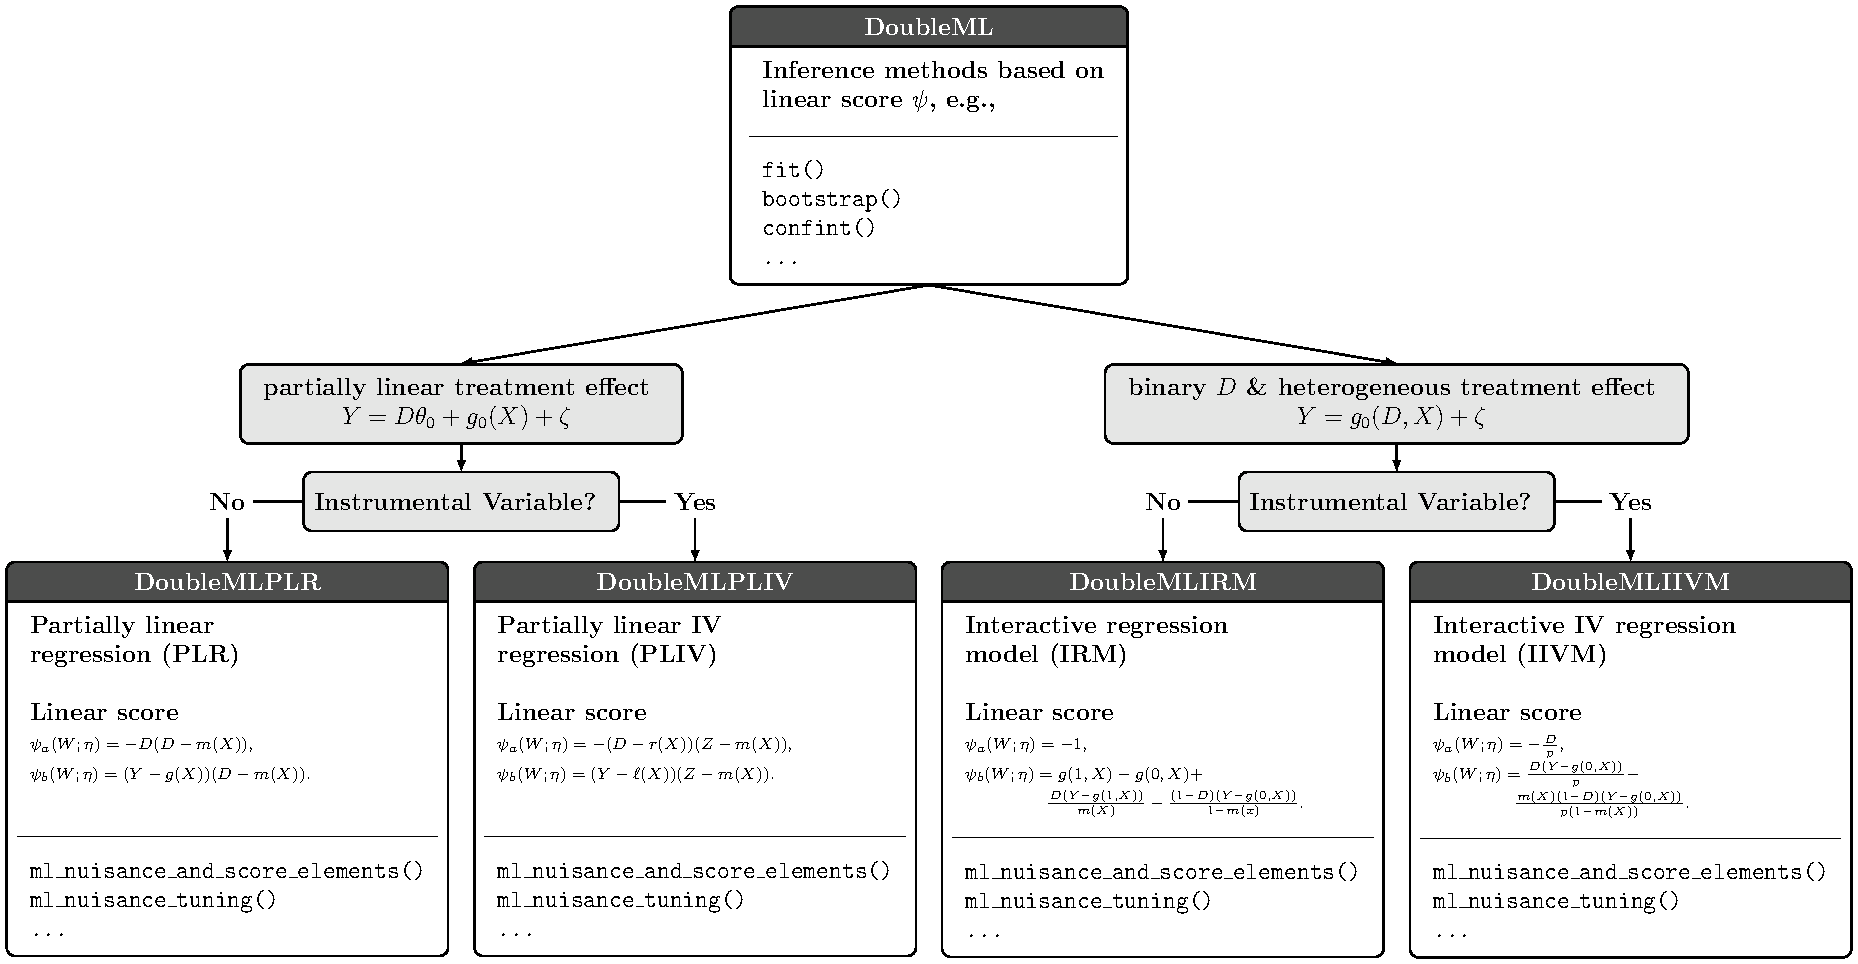
\includegraphics[width = 1\textwidth]{workflow/doubleml_models_with_linear_score_classes_methods.pdf}}{The figure shows a diagramm of the object class structure in DoubleML. On top, there is a box illustrating the base class DoubleML. In this class, inference methods that are based on a linear score function PSI are implemented, for example the methods fit() and confint() for parameter estimation and construction of confidence intervals. Below, there are four different boxes indiciating four different model classes: DoubleMLPLR for partially linear regression models, DoubleMLPLIV for partially linear instrumental variable regression, DoubleMLIRM for an interactive or nonparametric regression  model and DoubleMLIIVM for an IV-version of this interactive regression model. Each of these models is characterized by a different score function PSI.}
\end{center}

\end{frame}


\begin{frame}
\frametitle{Advantages of the Object-Orientation}
\begin{itemize}
\item \texttt{DoubleML} gives the user a \textbf{high flexibility} with regard to the specification of DML models:
\begin{itemize}
\item Choice of ML methods for approximating the nuisance functions
\item Different resampling schemes (repeated cross-fitting)
\item DML algorithms DML1 and DML2
\item Different Neyman orthogonal score functions
\end{itemize}
\item \texttt{DoubleML} can be \textbf{easily extended}
\begin{itemize}
\item New model classes with appropriate Neyman orthogonal score function can be inherited from \texttt{DoubleML}
\item The package features \texttt{callables} as score functions which makes it easy to extend existing model classes
\item The resampling schemes are customizable in a flexible way
\end{itemize}
\end{itemize}

\end{frame}



\mode<all>
\mode*

\begin{frame}
\frametitle{Online Resources}

\begin{center}
\pdftooltip{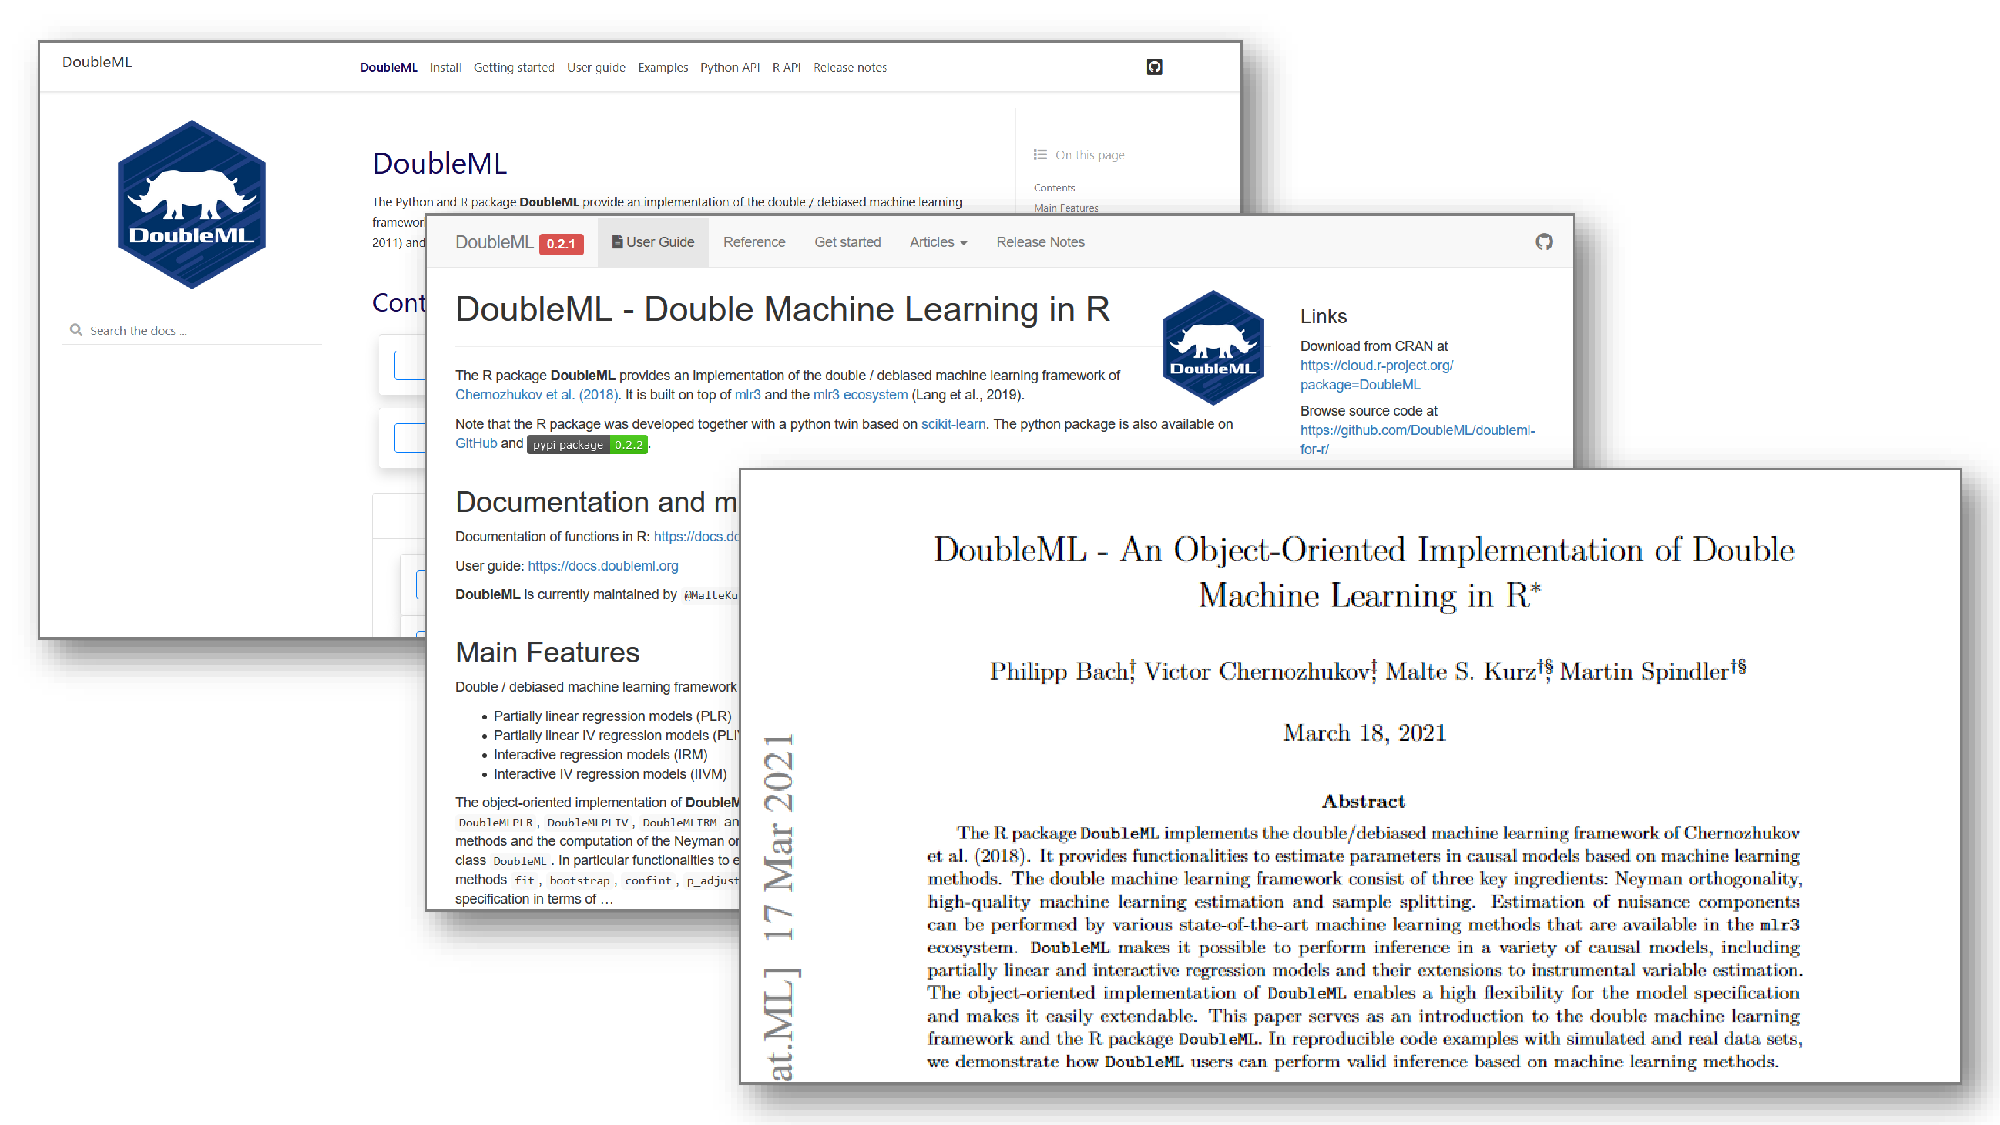
\includegraphics[width=0.8\textwidth]{pictures_and_logos/comingsoon_v3.pdf}}{An arrangement of three screenshots. The first screenshot on the left is a preview on the package website and user guide at https://docs.doubleml.org. The second screenshot which is in the middle is a preview on the documentation website of the R package available at https://docs.doubleml.org/r/stable/. The third screenshot (on the right) is a preview on the package vignette that is available at arxiv.}
\end{center}

\begin{itemize}
\item Documentation and User Guide available at
\begin{center}
\textbf{\url{https://docs.doubleml.org}}
\end{center}
\item Package vignette available via \href{https://arxiv.org/abs/2103.09603}{\textbf{arXiv:2103.09603}}
%\href{https://cran.r-project.org/web/packages/DoubleML/index.html}{\textbf{CRAN}} or
\end{itemize}
\end{frame}


\begin{frame}
\frametitle{Thank you, UseR!}

\begin{center}
\begin{large}
\textbf{Thank you very much for your attention!}
\end{large}
\end{center}
\vspace{20pt}
\begin{center}
\href{mailto:philipp.bach@uni-hamburg.de}{philipp.bach@uni-hamburg.de}\\
\href{mailto:malte.simon.kurz@uni-hamburg.de}{malte.simon.kurz@uni-hamburg.de}
\end{center}
\vspace{20pt}
\begin{center}
In case you like our project, we appreciate stars on GitHub :-) \\ \href{https://github.com/DoubleML/doubleml-for-r}{\texttt{https://github.com/DoubleML/doubleml-for-r}} 
\end{center}
%Documentation and User Guide available at \\
%\textbf{\url{https://docs.doubleml.org/}} \\
%\vspace{10pt}
%Package vignette available via\\ \href{https://arxiv.org/abs/2103.09603}{\textbf{arxiv}}
%% \href{https://cran.r-project.org/web/packages/DoubleML/index.html}{\textbf{CRAN}} or 
%\end{center}

\end{frame}


\begin{frame}
\frametitle{DoubleML: Package Papers}
\begin{itemize}
\item \textbf{Papers / Vignette}
\end{itemize}
\begin{beamercolorbox}[wd=\textwidth,rounded=true,shadow=true]{block body example}
\contrItemNormalSize{bach2021doublemlR}{DoubleML_Rhino_1000x1000.png}{r_logo.png}
\end{beamercolorbox}
\begin{beamercolorbox}[wd=\textwidth,rounded=true,shadow=true]{block body example}
\contrItemNormalSize{bach2021doublemlPy}{DoubleML_Rhino_1000x1000.png}{py_logo.png}
\end{beamercolorbox}
\vspace*{10pt}
%\begin{itemize}
%\item \textbf{User Guide} \url{https://docs.doubleml.org}
%\end{itemize}
%\begin{columns}
%\hspace*{12pt}
%\begin{column}{0.5\textwidth}
%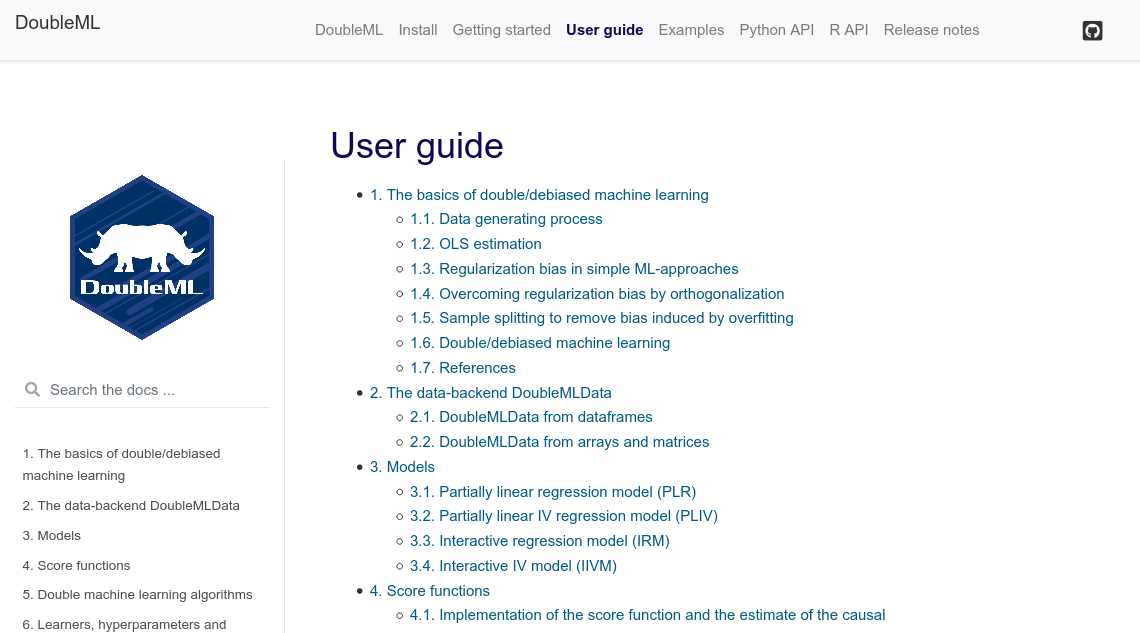
\includegraphics[width = 0.9\textwidth]{pictures_and_logos/user_guide_screenshot.png}
%\end{column}
%\begin{column}{0.5\textwidth}
%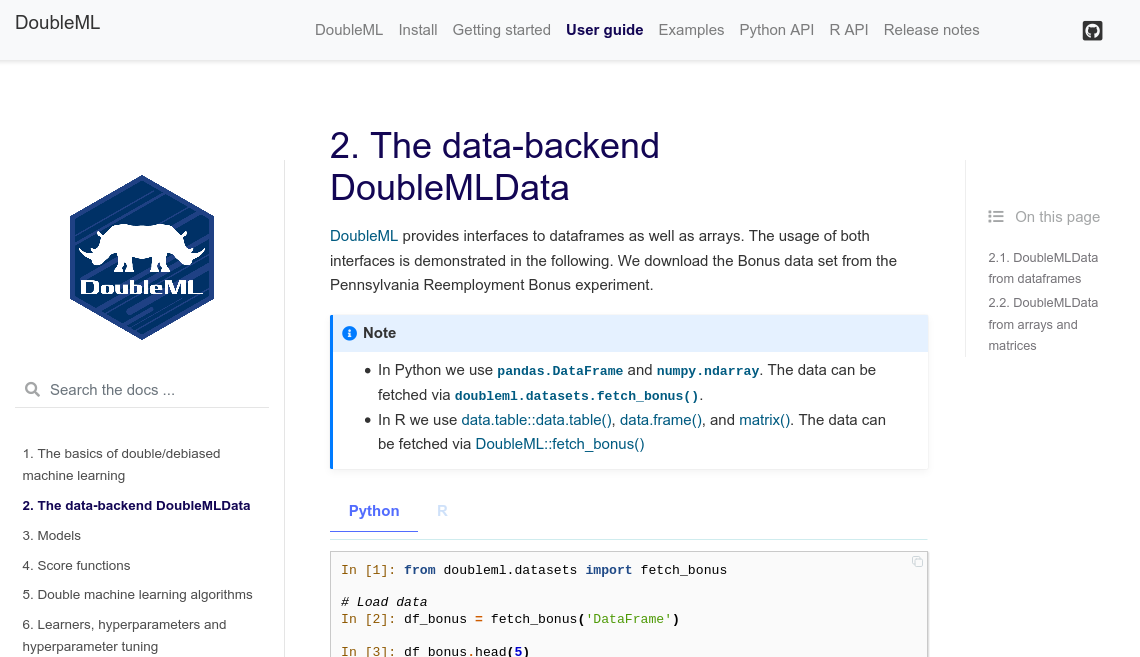
\includegraphics[width = 0.9\textwidth]{pictures_and_logos/user_guide_screenshot2.png}
%\end{column}
%\end{columns}
\end{frame}


\begin{frame}
\frametitle{References}
\renewcommand*{\bibfont}{\scriptsize}
\printbibliography
\end{frame}

\hypertarget{dml_workflow}{%
\section{Appendix: DoubleML Workflow}\label{dml_workflow}}

\mode<all>
\begin{frame}[fragile]
\frametitle{DoubleML Workflow: 0. Problem Formulation}
\begin{columns}
\begin{column}{0.3\textwidth}
\pdftooltip{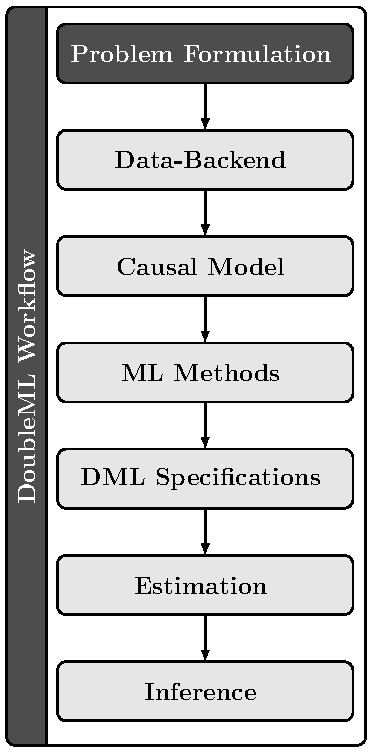
\includegraphics[width = \textwidth]{workflow/doubleml_workflow_problem.pdf}}{Description of Figure (alt-text): On the left hand side of the slide (and the following slides), there is a diagramm showing the seven steps of the DoubleML workflow. The fist step is the "Problem Formulation". The second step is the "Data-Backend". The third step is the "Causal Model". The fourth step is the choice of  "ML Methods". The fifth step is "DML Specifications". The sixth step is performing the "Estimation". The last step is then "Inference". In the following slides, each of the steps is explained in more detail. On each slide, the box of the corresponding workflow step is highlighted.}
\end{column}
\begin{column}{0.7\textwidth}
\textbf{Description of the Case Study and Data I}
\begin{itemize}
\small
\item 401(k) plans are pension accounts sponsored by employers
\item \textbf{Estimate the effect of 401(k) eligibility and participation on accumulated assets}
\item Problems: \textbf{Saver heterogeneity} and the fact that the \textbf{decision to enroll} in a 401(k) \textbf{is non-random}
\item \textbf{Conventional estimates} that do not account for saver heterogeneity and endogeneity of participation \textbf{will be biased}
\end{itemize}
\end{column}
\end{columns}
\end{frame}

\begin{frame}[fragile]
\frametitle{DoubleML Workflow: 0. Problem Formulation}
\begin{columns}
\begin{column}{0.3\textwidth}
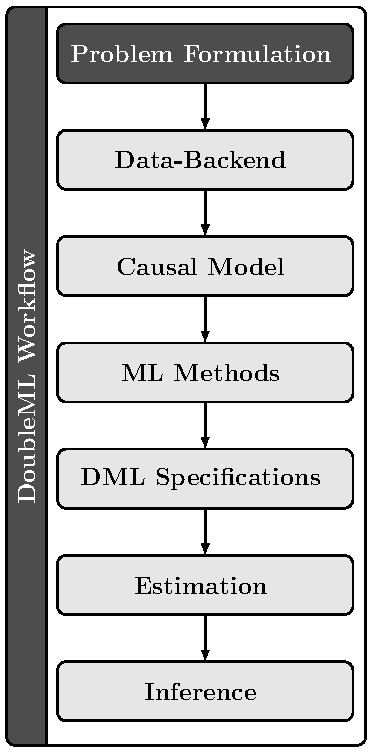
\includegraphics[width = \textwidth]{workflow/doubleml_workflow_problem.pdf}
\end{column}
\begin{column}{0.7\textwidth}
\textbf{Description of the Case Study and Data II}
\begin{itemize}
\small
\item \textbf{Eligibility} for enrolling in a 401(k) plan might be taken as \textbf{exogenous after conditioning} on a few observables of which the most important may be income
\item \textbf{The basic idea}:  Around the time 401(k)’s initially became available, people were unlikely to be basing their employment decisions on whether an employer offered a 401(k) but would instead focus on income and other aspects of the job
\item The data consist of 9,915 observations at the household level drawn from the 1991 Survey of Income and Program Participation (SIPP)
\item \textbf{Outcome variable: Net financial assets}
\end{itemize}
\end{column}
\end{columns}
\end{frame}

\begin{frame}[fragile]
\frametitle{DoubleML Workflow: 1. Data-Backend}
\begin{columns}
\begin{column}{0.3\textwidth}
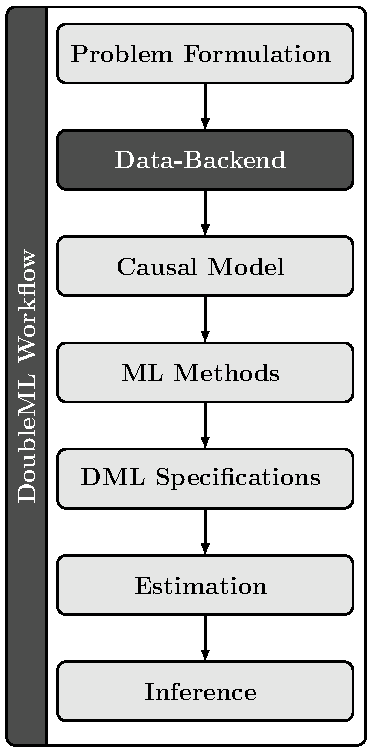
\includegraphics[width = \textwidth]{workflow/doubleml_workflow_data.pdf}
\end{column}
\begin{column}{0.7\textwidth}
\begin{itemize}
\item \textbf{DoubleMLData} from a data.table or data.frame
\end{itemize}
{\tiny
\begin{lstlisting}[language=Python,
backgroundcolor = \color{gray!20},
keywordstyle=\color{OliveGreen}, stringstyle=\color{BrickRed}]
library(DoubleML)
data = fetch_401k(return_type='data.table')
# Construct DoubleMLData object from data.table
dml_data = DoubleMLData$new(data, y_col='net_tfa', d_cols='e401',
	                    x_cols=c('age', 'inc', 'educ', 'fsize',
	                             'marr', 'twoearn', 'db', 'pira',
	                             'hown'))
	                        		 
data_frame = fetch_401k(return_type='data.frame')
# Construct DoubleMLData object from data.frame
dml_data_df = double_ml_data_from_data_frame(data_frame,
                                             y_col='net_tfa',
                                             d_cols='e401', 
                                             x_cols=c('age', 'inc',
                                                      'educ', 'fsize',
                                                      'marr', 'twoearn',
                                                      'db', 'pira',
                                                      'hown'))
\end{lstlisting}
}
\begin{itemize}
\item \textbf{DoubleMLData} from matrix
\end{itemize}
{\tiny
\begin{lstlisting}[language=Python,
backgroundcolor = \color{gray!20},
keywordstyle=\color{OliveGreen}, stringstyle=\color{BrickRed}]
# Simulate data
set.seed(3141); n_obs = 500; n_vars = 100; theta = 3; 
X = matrix(rnorm(n_obs*n_vars), nrow=n_obs, ncol=n_vars)
d = X[,1:3]%*%c(5,5,5) + rnorm(n_obs)
y = theta*d + X[, 1:3]%*%c(5,5,5) + rnorm(n_obs)

dml_data_sim =  double_ml_data_from_matrix(X, y, d)
\end{lstlisting}
}
\end{column}
\end{columns}
\end{frame}

\begin{frame}
\frametitle{DoubleML Workflow: 2. Causal Model}
\begin{columns}
\begin{column}{0.3\textwidth}
\pdftooltip{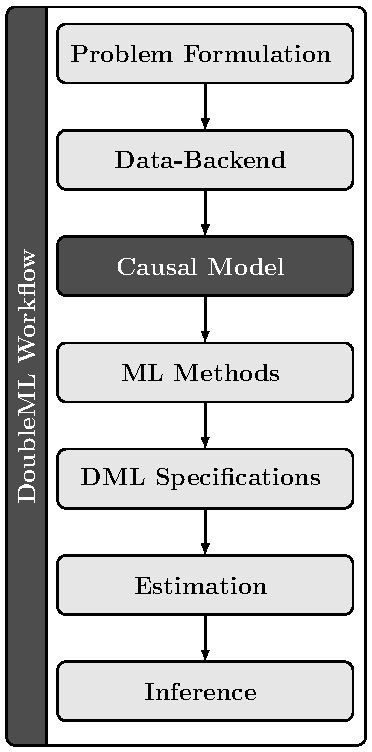
\includegraphics[width = \textwidth]{workflow/doubleml_workflow_causal.pdf}}{The figure shows a diagramm of the causal models that are currently implemented in DoubleML. On top, there is a box with annotation "DoubleML Models". From this box, two arrows go out into two boxes that are located on a layer below. In the box on the left hand side, it is written "partially linear treatment effect" with the formula for a partially linear regression model and an additive causal effect THETANULL associated with variable D. In the box on the right hand side, it is written "binary D and heterogeneous treatment effect" with a formula for a non-parameteric regression model. Each of the two boxes has an arrow going to a box with the question "Instrumental Variable?". If the answer to this question is yes, the arrows goes into the respective box that represents each of the causal models: The partially linear regression model without instrumental model called the "Partially linear regression (PLR) or the model with instrumental variable. The latter is called the "Partially linear IV regression (PLIV)". On the right hand side, the model without instrumental variable is called the "Interactive regression model (IRM)". The model with instrumental variable is called the "Interactive IV model (IIVM)".}
\end{column}
\begin{column}{0.7\textwidth}
\begin{itemize}
\item Specify a \textbf{causal model}
\end{itemize}
\vspace*{10pt}
\hspace*{-0.7cm}
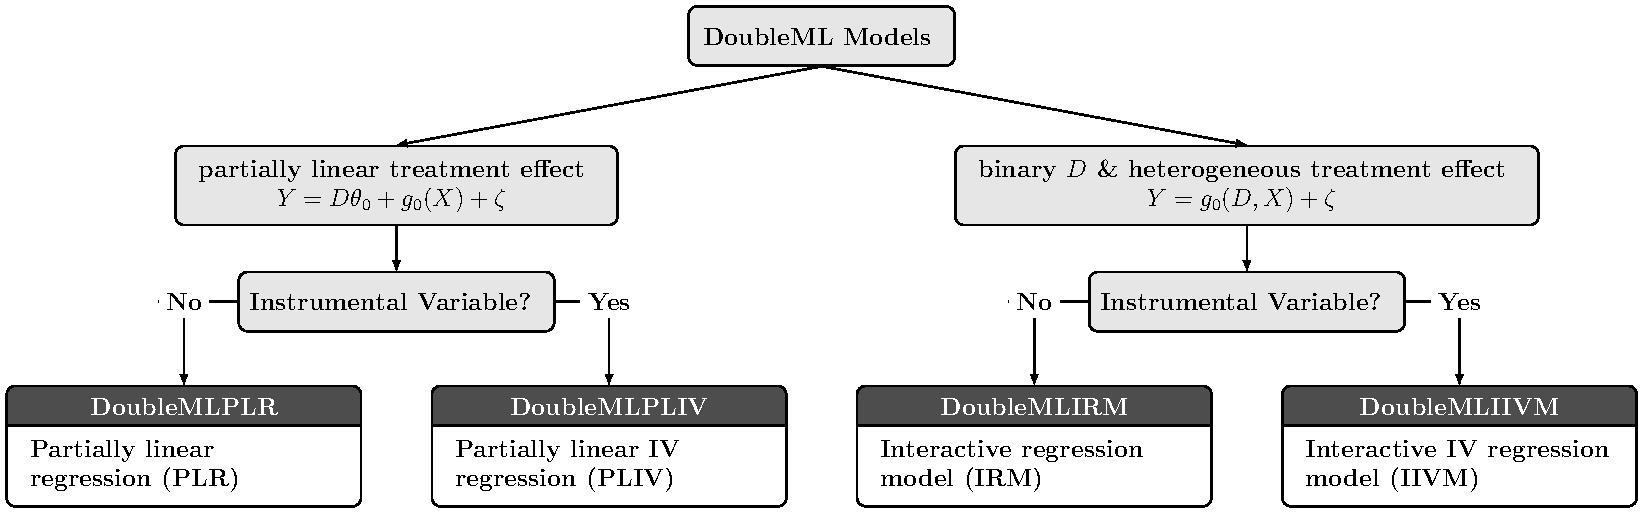
\includegraphics[width=1.17\textwidth]{workflow/doubleml_models.pdf}
\begin{itemize}
\item 401k data: Partially linear regression (PLR)
\end{itemize}
\vspace*{10pt}
\begin{center}
\pdftooltip{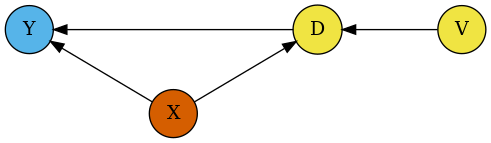
\includegraphics[width=0.8\textwidth]{pictures_and_logos/dag_plr2.png}}{A graph illustrating the  partially linear regression setting. There are four nodes in total: One for the dependent variable Y, one for the treatment variable D, one for the vector of confounding variables X and one for the stochastic error V. There are four directed edges in the figure, each illustrating a causal channel: From V into D, from D into Y, from X into Y and from X into D.}
\end{center}
\end{column}
\end{columns}
\end{frame}

\begin{frame}[fragile]
\frametitle{DoubleML Workflow: 3. ML Methods}
\begin{columns}
\begin{column}{0.3\textwidth}
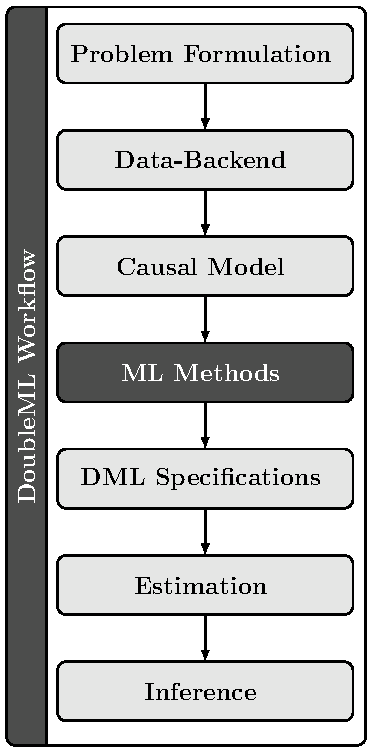
\includegraphics[width = \textwidth]{workflow/doubleml_workflow_ml.pdf}
\end{column}
\begin{column}{0.7\textwidth}
\begin{itemize}
\item Choose \textbf{ML methods} to approximate the nuisance functions
\item PLR
\begin{itemize}
\item $g_0(X) = \mathbb{E}(Y|X)$
\item $m_0(X) = \mathbb{E}(D|X)$
\end{itemize}
\item Random forest from ranger/mlr3learners.
\end{itemize}
{\tiny
\begin{lstlisting}[language=Python,
backgroundcolor = \color{gray!20},
keywordstyle=\color{OliveGreen}, stringstyle=\color{BrickRed}]
library(mlr3learners)
ml_g_rf = lrn("regr.ranger", max.depth = 7,
              mtry = 3, min.node.size = 3)
ml_m_rf = lrn("classif.ranger", max.depth = 5,
              mtry = 4, min.node.size = 7)
\end{lstlisting}
}
\begin{itemize}
\item Boosted trees from xgboost/mlr3extralearners
\end{itemize}
{\tiny
\begin{lstlisting}[language=Python,
backgroundcolor = \color{gray!20},
keywordstyle=\color{OliveGreen}, stringstyle=\color{BrickRed}]
ml_g_xgb = lrn("regr.xgboost",
               objective = "reg:squarederror",
               eta = 0.1, nrounds = 35)
ml_m_xgb = lrn("classif.xgboost",
               objective = "binary:logistic",
               eval_metric = "logloss",
               eta = 0.1, nrounds = 34)
\end{lstlisting}
}
\end{column}
\end{columns}
\end{frame}

\begin{frame}[fragile]
\frametitle{DoubleML Workflow: 4. DML Specifications}
\begin{columns}
\begin{column}{0.3\textwidth}
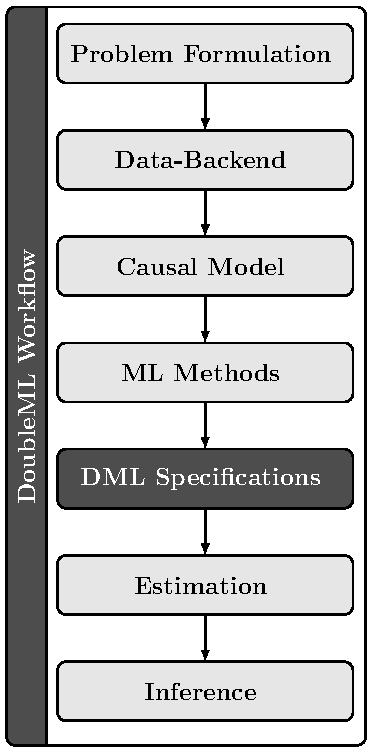
\includegraphics[width = \textwidth]{workflow/doubleml_workflow_dml.pdf}
\end{column}
\begin{column}{0.7\textwidth}
\begin{itemize}
\item \textbf{Initialize a DoubleMLPLR model}
\end{itemize}
{\tiny
\begin{lstlisting}[language=Python,
backgroundcolor = \color{gray!20},
keywordstyle=\color{OliveGreen}, stringstyle=\color{BrickRed}]
set.seed(123)
dml_plr_forest = DoubleMLPLR$new(dml_data,
                                 ml_g = ml_g_rf,
                                 ml_m = ml_m_rf,
                                 n_folds = 3)
\end{lstlisting}
}
\begin{itemize}
\item \textbf{Parametrize DoubleML models}
\begin{itemize}
\item \textbf{Resampling} (repeated cross-fitting): Number of repetitions \& folds
\item \textbf{DML algorithm}: dml1 vs.\ dml2
\item Neyman orthogonal \textbf{score function} (for PLR 'partialling out' or 'IV-type')
\end{itemize}
\end{itemize}
{\tiny
\begin{lstlisting}[language=Python,
backgroundcolor = \color{gray!20},
keywordstyle=\color{OliveGreen}, stringstyle=\color{BrickRed}]
set.seed(123)
dml_plr_forest = DoubleMLPLR$new(dml_data, ml_g = ml_g_rf,
                                 ml_m = ml_m_rf, n_folds=3, n_rep=1,
                                 score='partialling out',
                                 dml_procedure='dml2')
\end{lstlisting}
}
\end{column}
\end{columns}
\end{frame}

\begin{frame}[fragile]
\frametitle{DoubleML Workflow: 5. Estimation}
\begin{columns}
\begin{column}{0.3\textwidth}
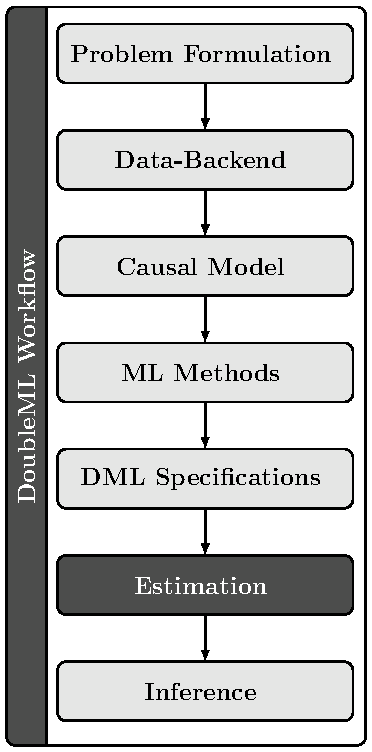
\includegraphics[width = \textwidth]{workflow/doubleml_workflow_est.pdf}
\end{column}
\begin{column}{0.7\textwidth}
\begin{itemize}
\item \textbf{Estimation} of the DoubleML model
\end{itemize}
{\tiny
\begin{lstlisting}[language=Python,
backgroundcolor = \color{gray!20},
keywordstyle=\color{OliveGreen}, stringstyle=\color{BrickRed}]
dml_plr_forest$fit()
\end{lstlisting}
}
\begin{itemize}
\item Estimated causal effect
\end{itemize}
{\tiny
\begin{lstlisting}[language=Python,
backgroundcolor = \color{gray!20},
keywordstyle=\color{OliveGreen}, stringstyle=\color{BrickRed}]
dml_plr_forest$coef
    e401 
8968.788
\end{lstlisting}
}
\begin{itemize}
\item Estimated standard error
\end{itemize}
{\tiny
\begin{lstlisting}[language=Python,
backgroundcolor = \color{gray!20},
keywordstyle=\color{OliveGreen}, stringstyle=\color{BrickRed}]
dml_plr_forest$se
    e401 
1341.061 
\end{lstlisting}
}
\begin{itemize}
\item \textbf{Summary} of the estimated effect
\end{itemize}
{\tiny
\begin{lstlisting}[language=Python,
backgroundcolor = \color{gray!20},
keywordstyle=\color{OliveGreen}, stringstyle=\color{BrickRed}]
dml_plr_forest$summary()
[1] "Estimates and significance testing of the effect of target variables"
     Estimate. Std. Error t value Pr(>|t|)    
e401      8969       1341   6.688 2.27e-11 ***
---
Signif. codes:  0 '***' 0.001 '**' 0.01 '*' 0.05 '.' 0.1 ' ' 1
\end{lstlisting}
}
\end{column}
\end{columns}
\end{frame}

\begin{frame}[fragile]
\frametitle{DoubleML Workflow: 6. Inference}
\begin{columns}
\begin{column}{0.3\textwidth}
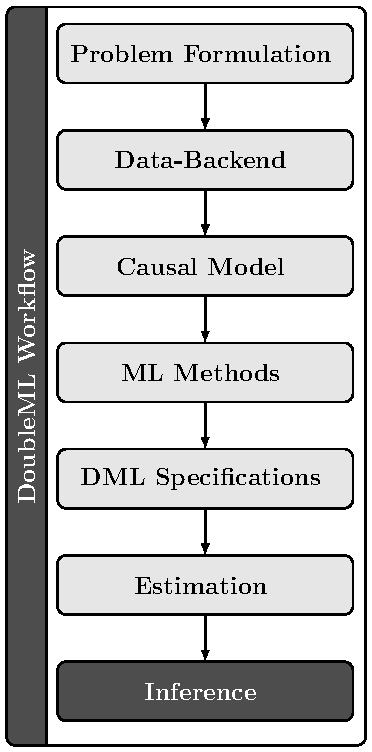
\includegraphics[width = \textwidth]{workflow/doubleml_workflow_inf.pdf}
\end{column}
\begin{column}{0.7\textwidth}
\begin{itemize}
\item Summary of the estimated effect
\end{itemize}
{\tiny
\begin{lstlisting}[language=Python,
backgroundcolor = \color{gray!20},
keywordstyle=\color{OliveGreen}, stringstyle=\color{BrickRed}]
dml_plr_forest$summary()
[1] "Estimates and significance testing of the effect of target variables"
     Estimate. Std. Error t value Pr(>|t|)    
e401      8969       1341   6.688 2.27e-11 ***
---
Signif. codes:  0 '***' 0.001 '**' 0.01 '*' 0.05 '.' 0.1 ' ' 1

\end{lstlisting}
}
\begin{itemize}
\item \textbf{Confidence interval(s)}
\end{itemize}
{\tiny
\begin{lstlisting}[language=Python,
backgroundcolor = \color{gray!20},
keywordstyle=\color{OliveGreen}, stringstyle=\color{BrickRed}]
dml_plr_forest$confint()
        2.5 %   97.5 %
e401 6340.356 11597.22
\end{lstlisting}
}
\begin{itemize}
\item \textbf{Multiplier bootstrap} \\
$\rightarrow$ relevant for multiple treatment effects!
\end{itemize}
{\tiny
\begin{lstlisting}[language=Python,
backgroundcolor = \color{gray!20},
keywordstyle=\color{OliveGreen}, stringstyle=\color{BrickRed}]
dml_plr_forest$bootstrap()
\end{lstlisting}
}
\begin{itemize}
\item Confidence interval(s) based on the multiplier bootstrap
\end{itemize}
{\tiny
\begin{lstlisting}[language=Python,
backgroundcolor = \color{gray!20},
keywordstyle=\color{OliveGreen}, stringstyle=\color{BrickRed}]
dml_plr_forest$confint(joint=TRUE)
        2.5 %   97.5 %
e401 6174.467 11763.11
\end{lstlisting}
}
\end{column}
\end{columns}
\end{frame}


%
%
%\begin{frame}[fragile]
%\frametitle{DoubleML API: R vs. Python}
%\begin{columns}
%\begin{column}{0.5\textwidth}
%\begin{block}{R}
%{\tiny
%\begin{lstlisting}[language=R, keywords={library},
%keywordstyle=\color{MidnightBlue}, stringstyle=\color{OliveGreen}]
%library(DoubleML)
%library(mlr3)
%library(mlr3learners)
%set.seed(1234)
%
%
%data_plr = make_plr_CCDDHNR2018(
%  alpha = 0.5, n_obs = 500, dim_x = 20,
%  return_type = 'data.table')
%obj_dml_data = DoubleMLData$new(
%  data_plr, y_col = 'y', d_cols = 'd')
%
%ml_g = lrn("regr.ranger")
%ml_m = lrn("regr.ranger")
%doubleml_plr = DoubleMLPLR$new(
%  obj_dml_data, ml_g, ml_m,
%  n_folds = 2, score = 'partialling out')
%
%doubleml_plr$fit()
%doubleml_plr$summary()
%   Estimate.  Std. Error  t value  Pr(>|t|)    
%d  0.51982    0.04061     12.8     <2e-16   ***
%\end{lstlisting}
%}
%\end{block}
%\end{column}
%\begin{column}{0.5\textwidth}
%\begin{block}{Python}
%{\tiny
%\begin{lstlisting}[language=Python,
%keywordstyle=\color{OliveGreen}, stringstyle=\color{BrickRed}]
%from doubleml import DoubleMLData, DoubleMLPLR
%from doubleml.datasets import make_plr_CCDDHNR2018
%import numpy as np
%from sklearn.ensemble import RandomForestRegressor
%np.random.seed(1234)
%
%data_plr = make_plr_CCDDHNR2018(
%    alpha = 0.5, n_obs = 500, dim_x = 20,
%    return_type = 'DataFrame')
%obj_dml_data = DoubleMLData(
%    data_plr, y_col = 'y', d_cols = 'd')
%
%ml_g = RandomForestRegressor()
%ml_m = RandomForestRegressor()
%doubleml_plr = DoubleMLPLR(
%    obj_dml_data, ml_g, ml_m,
%    n_folds = 2, score = 'partialling out')
%
%doubleml_plr.fit()
%doubleml_plr.summary
%  coef   std err t      P>|t| 2.5 % 97.5 %
% d 0.534 0.042   12.669 0.0   0.451 0.617
%\end{lstlisting}
%}
%\end{block}
%\end{column}
%\end{columns}
%
%\end{frame}



\end{document}
